\documentclass{beamer}


\usepackage[french,english]{babel}

\usepackage[T1]{fontenc}

\usepackage[utf8]{inputenc}


\usetheme{Warsaw}
\title{Apprentissage et résultats}

\author{Clément Legrand}

\begin{document}


\begin{frame}[plain]
\titlepage
\end{frame}

\section{Apprentissage}

\subsection{Description}

\begin{frame}{Description}
\begin{block}{Base de départ}
Les solutions données par CW.
\begin{itemize}
\item Tirage au sort de N triplets ($\lambda$, $\mu$, $\nu$);
\item Calcul de toutes les solutions possibles.
\end{itemize}
\end{block}

\begin{block}{Base d'apprentissage}
On peut ne garder qu'une partie de la base générée pour apprendre
\begin{itemize}
\item On garde $x\%$ des meilleurs solutions (quantité privilégiée, Quan$_{x}$);
\item On garde les solutions qui ont un coût inférieur à $c_{min} + (c_{max}-c_{min})\frac{x}{100}$ (qualité privilégiée, Qual$_{x}$).
\item On choisit d'utiliser toute la base générée pour apprendre (Tout)
\end{itemize}
\end{block}
\end{frame}

\begin{frame}{Protocole}

\begin{exampleblock}{Protocole}
\begin{itemize}
\item Génération de la base de départ
\item Génération de la base d'apprentissage
\item On initialise une matrice MAT de taille $n^2$
\item Pour chaque arête (a,b) on incrémente la valeur MAT[a][b] (si a>b, on commence par échanger a et b)
\item On regarde si les arêtes obtenues sont effectivement dans la solution optimale.
\end{itemize}
\end{exampleblock}

\begin{block}{Choix des arêtes}
\begin{itemize}
\item On conserve (a,b) si MAT[a][b] dépasse une certaine valeur (Seuil);
\item On conserve les k premières arêtes en triant selon les valeurs contenues dans MAT (Rang).
\end{itemize}
\end{block}

\end{frame}

\subsection{Résultats apprentissage}

\begin{frame}{Instance test}
Tous les tests qui suivent n'ont été réalisés que sur l'instance A-n37-k06.

La solution employée pour comparer les résultats est celle de la littérature.

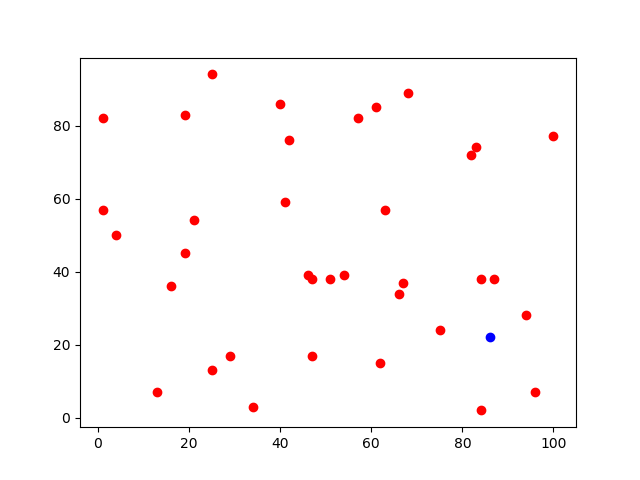
\includegraphics[scale=0.3]{instance3706.png}
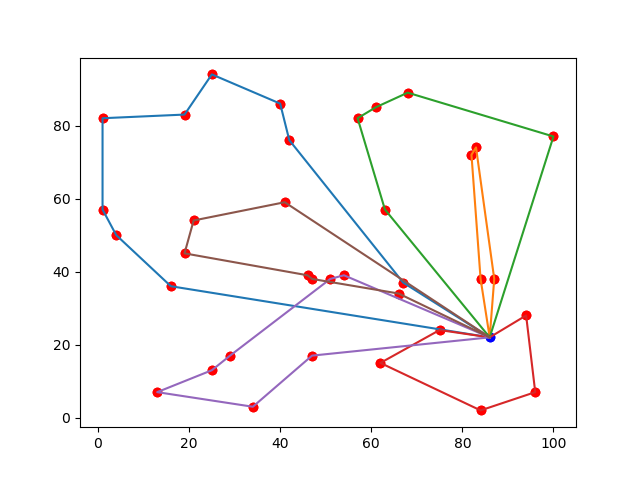
\includegraphics[scale=0.3]{best3706.png}

Pour chaque test on effectue 5 itérations.
\end{frame}

\begin{frame}{Résultats avec critère Seuil et Quan$_{10}$}
\emph{L$_{lb}$} est la taille de la base d'apprentissage. 

La meilleure solution comporte 42 arêtes.

On utilise la méthode Quan$_{10}$ avec certaines valeurs de seuil.

\begin{tabular}{|c|c|c|c|c|}
   \hline
   Taille base & Seuil & Nb arêtes & Nb correctes & Proportion\\
   \hline
   100 & L$_{lb}$/2 & 30 & 21 & 0.5  \\
   \hline
   500 & L$_{lb}$/2 & 32 & 24 & 0.57  \\
   \hline
   1000 & L$_{lb}$/2 & 33 & 24 & 0.57  \\
   \hline
   \hline
   100 & 3L$_{lb}$/4 & 16 & 15 & 0.36  \\
   \hline
   500 & 3L$_{lb}$/4 & 15 & 14 & 0.33  \\
   \hline
   1000 & 3L$_{lb}$/4 & 16 & 14 & 0.33  \\
   \hline
\end{tabular}


\end{frame}

\begin{frame}{Résultats Seuil avec Qual$_{10}$}
On utilise la méthode Qual$_{10}$ avec certaines valeurs de seuil.
\begin{tabular}{|c|c|c|c|c|}
   \hline
   Taille base & Seuil & Nb arêtes & Nb correctes & Proportion\\
   \hline
   100 & L$_{lb}$/2 & 31 & 23 & 0.55  \\
   \hline
   500 & L$_{lb}$/2 & 31 & 22 & 0.52  \\
   \hline
   1000 & L$_{lb}$/2 & 31 & 23 & 0.53  \\
   \hline
   \hline
   100 & 3L$_{lb}$/4 & 17 & 14 & 0.33  \\
   \hline
   500 & 3L$_{lb}$/4 & 20 & 16 & 0.38  \\
   \hline
   1000 & 3L$_{lb}$/4 & 19 & 16 & 0.38  \\
   \hline
\end{tabular}
\end{frame}

\begin{frame}{Résultats Seuil avec Tout}
On utilise la méthode Tout avec certaines valeurs de seuil.
\begin{tabular}{|c|c|c|c|c|}
   \hline
   Taille base & Seuil & Nb arêtes & Nb correctes & Proportion\\
   \hline
   100 & L$_{lb}$/2 & 24 & 17 & 0.40  \\
   \hline
   500 & L$_{lb}$/2 & 22 & 15 & 0.36  \\
   \hline
   1000 & L$_{lb}$/2 & 23 & 16 & 0.38  \\
   \hline
   \hline
   100 & 3L$_{lb}$/4 & 6 & 6 & 0.14  \\
   \hline
   500 & 3L$_{lb}$/4 & 7 & 7 & 0.18  \\
   \hline
   1000 & 3L$_{lb}$/4 & 6 & 6 & 0.14  \\
   \hline
\end{tabular}
\end{frame}

\begin{frame}{Bilan avec critère Seuil}

\begin{itemize}
\item Quan$_{10}$ et Qual$_{10}$ renvoient en moyenne 22 arêtes correctes lorsque Seuil vaut L$_{lb}$/2, et 15 lorsque Seuil vaut 3L$_{lb}$/4;
\item Tout renvoie en moyenne respectivement 15 et 6 arêtes correctes.
\end{itemize}

\begin{exampleblock}{Remarque}
Quan$_{10}$ semble être la base la plus adaptée pour le critère de choix Requis.
\end{exampleblock}

\end{frame}

\begin{frame}{Résultats avec critère Rang et Quan$_{10}$}

On utilise la méthode Quan$_{10}$ avec certaines valeurs de rang.
\begin{tabular}{|c|c|c|c|}
   \hline
   Taille base & Rang max & Nb correctes & Proportion\\
   \hline
   100 & 10  & 9 & 0.21  \\
   \hline
   500 & 10  & 9 & 0.21  \\
   \hline
   1000 & 10 & 9 & 0.21  \\
   \hline
   \hline
   100 & 20 & 16 & 0.38  \\
   \hline
   500 & 20 & 16 & 0.38  \\
   \hline
   1000 & 20 & 17 & 0.40  \\
   \hline
\end{tabular}

\end{frame}

\begin{frame}{Résultats avec critère Rang et Qual$_{10}$}

On utilise la méthode Qual$_{10}$ avec certaines valeurs de rang.
\begin{tabular}{|c|c|c|c|}
   \hline
   Taille base & Rang max & Nb correctes & Proportion\\
   \hline
   100 & 10  & 9 & 0.21  \\
   \hline
   500 & 10  & 10 & 0.24  \\
   \hline
   1000 & 10 & 10 & 0.24  \\
   \hline
   \hline
   100 & 20 & 16 & 0.38  \\
   \hline
   500 & 20 & 16 & 0.38  \\
   \hline
   1000 & 20 & 16 & 0.38  \\
   \hline
\end{tabular}
\end{frame}

\begin{frame}{Résultats avec critère Rang et Tout}

On utilise la méthode Tout avec certaines valeurs de rang.
\begin{tabular}{|c|c|c|c|}
   \hline
   Taille base & Rang max & Nb correctes & Proportion\\
   \hline
   100 & 10  & 10 & 0.24  \\
   \hline
   500 & 10  & 9 & 0.21  \\
   \hline
   1000 & 10 & 10 & 0.24  \\
   \hline
   \hline
   100 & 20 & 15 & 0.36  \\
   \hline
   500 & 20 & 15 & 0.36  \\
   \hline
   1000 & 20 & 15 & 0.36  \\
   \hline
\end{tabular}
\end{frame}
\begin{frame}{Bilan avec critère Seuil}
\begin{exampleblock}{Remarque}
Qual$_{10}$ semble être la base la plus adaptée pour le critère de choix Rang.
\end{exampleblock}
\end{frame}

\begin{frame}{Résultats avec toutes les SI}
Temps de calcul pour avoir la base : 37.5 s

\centering
\begin{tabular}{|c|c|c|c|}
   \hline
   Requis & Rés Quan$_{10}$ & Rés Qual$_{10}$ & Time (s)\\
   \hline
   L$_{lb}$/2 & 33 - 24 - 0.57 & 30 - 23 - 0.55 & 0.076 \\
   \hline
   3L$_{lb}$/4 & 15 - 14 - 0.33 & 18 - 16 - 0.38  & 0.077 \\
   \hline
\end{tabular}

Quan$_{10}$ reste la base la plus performante pour le critère Requis.

\begin{tabular}{|c|c|c|c|}
   \hline
   Rang max & Rés Quan$_{10}$ & Rés Qual$_{10}$ & Time (s)\\
   \hline
   10 & 9 - 0.21 & 10 - 0.24 & 0.074 \\
   \hline
   20 & 17 - 0.40 & 17 - 0.40 & 0.076 \\
   \hline
\end{tabular}

Qual$_{10}$ reste la base la plus performante pour le critère Rang.
\end{frame}

\section{Intégration de la connaissance dans un algorithme}

\subsection{Présentation algorithme}
\begin{frame}{Algorithme actuel}

\begin{center}
\begin{tabular}{|c|}
	\hline
 	\textbf{Apprentissage} \\
   \hline
   Boucle sur $(\lambda, \nu, \mu)$ \\
   \hline
   \hline
   Initialisation$_{CW}$ + \textbf{utilisation apprentissage} \\
   \hline
   LK$_{BI-O}$ \\
   \hline
   \hline
   Condition d'arrêt : 1500 itérations depuis la dernière amélioration  \\
   \hline
   Compute worst edge \\
   \hline
   EC$_{BI-O}$ \\
   \hline
   LK$_{BI-O}$ \\
   \hline
   CE$_{FI-O}$ \\
   \hline
   LK$_{BI-O}$ \\
   \hline
   Itérations spéciales \\
   \hline
   \hline

\end{tabular}
\end{center}
\end{frame}

\subsection{Résultats}

\begin{frame}{Premiers résultats}

\begin{tabular}{|c|c|c|c|c|}
   \hline
   Méthode  & A-n34-k05 (779) & Time (s) & A-n37-k06 (952) & Time (s) \\
   \hline
   Sans & 781.96  & 614 & 950.85 & 1325  \\
   \hline
   Quan$_{10}$ & 795.88 & 56 & 950.85 & 1158   \\
   \hline
   Qual$_{10}$ & 788.98 & 495 & 951.85 & 601  \\
   \hline
\end{tabular}

\begin{tabular}{|c|c|c|}
   \hline
   Méthode  & A-n65-k09 (1182) & Time (s) \\
   \hline
   Quan$_{10}$ & 1189.64 & 2085    \\
   \hline
   Qual$_{10-10}$ & 1200.11 & 2442   \\
   \hline
   Qual$_{10-half}$ & 1183.31 & 2541  \\
   \hline
\end{tabular}

\begin{block}{Modifications}
\begin{itemize}
\item Changement Algorithme ?
\item Nouveau choix des paramètres ?
\end{itemize}
\end{block}

\end{frame}

\end{document}
